\documentclass[12pt]{article}

\usepackage[left=0.75in, right=0.75in, top=0.75in, bottom=0.75in]{geometry}
\setlength\parindent{0pt}

\usepackage{epsfig,graphics,amsmath,color,multicol,tcolorbox,enumitem}


\setlist{noitemsep}
\setlist{nolistsep}
\pagestyle{empty}

\begin{document}

\begin{tabular*}{\textwidth}{@{\extracolsep{\fill}}l l}
\textbf{Product and Quotient Rules }  & Derivative Apprentice:  \rule{6cm}{0.5pt} \\
MATH 160 & Section:\\
\hline\hline
\end{tabular*} \\

\small

Aligns with Standard D5 \rm

\hrulefill
\normalsize



\bigskip

\begin{enumerate}

\item Calculate the indicated derivatives using differentiation rules.  Do not simplify. And make sure you include parenthesis!
	\begin{enumerate}
	\item $\dfrac{d}{dx} (1+\sqrt{x}+x^2)(1-\frac{1}{2x}-x^3)$
	\vfill
	\item $\dfrac{d}{dt} \left[ \dfrac{t^3-3^t+e^t}{9-\pi-t} \right]$ 	\vfill
	\item $\dfrac{d}{dx} \cos(x)\ln(x)$
	\vfill
	\item $\dfrac{d}{dx} \dfrac{2^{x}}{\sin(x)x^9}$			\vfill

	\end{enumerate}


\item Use the following table to evaluate each derivative.\\\\


\begin{tabular}{c | c | c | c | c }
$x$ & $f(x)$ & $g(x)$ & $f'(x)$ & $g'(x)$ \\
\hline
0 & 1 & 1 & -3 & 0.5 \\
1 & 3 & 5 & 0.5 & -4
\end{tabular}

\begin{enumerate}
\begin{multicols}{2}
\item $h(x)=\dfrac{2f(x)}{g(x)}$.  Find $h'(0)$.
\vspace{2cm}
\item $p(x)=f(x)\cdot g(x) $.  Find $p'(1)$.
\vspace{2cm}
\end{multicols}
\end{enumerate}
\vspace{.5in}
\newpage

\item The graphs of $f\left(x\right)$ (red dashed) and $g\left(x\right)$ (blue solid) are graphed. Let $h(x)=f(x) \cdot g(x)$ and $j(x)=\frac{f(x)}{g(x)}$.  Use information about $f$ and $g$ to evaluate the derivatives below:

\begin{multicols}{2}

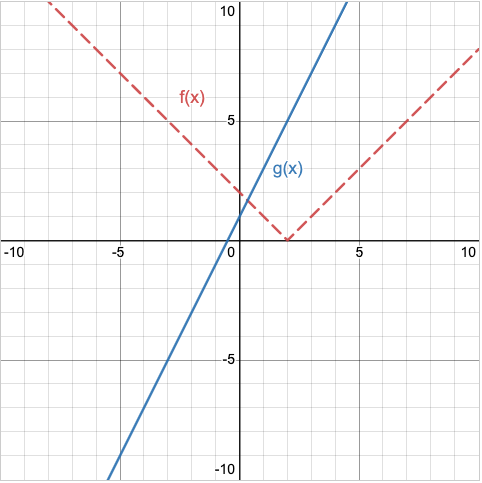
\includegraphics[scale=0.4]{fgOne.png}

\begin{enumerate}[parsep=1in]
\item Compute $h'(4)$. \vskip .75in
\item Compute $j'(4)$.
\end{enumerate}

\end{multicols}

\item Verify, using the quotient rule, that 
    $\displaystyle{\frac{d}{dx}\left[\tan(x)\right]=\sec^2(x)}$ (Hint: $\tan(x)=\frac{\sin(x)}{\cos(x)}$, $\sin^2(x)+\cos^2(x)=1$ and $\sec(x)=\frac{1}{\cos(x)}$)
	\vfill

\item From the Module 8 Quiz prep problem: If the graph below is of the {\bf derivative}, $f'(x)$, sketch a possible graph of the parent function, $f(x)$.

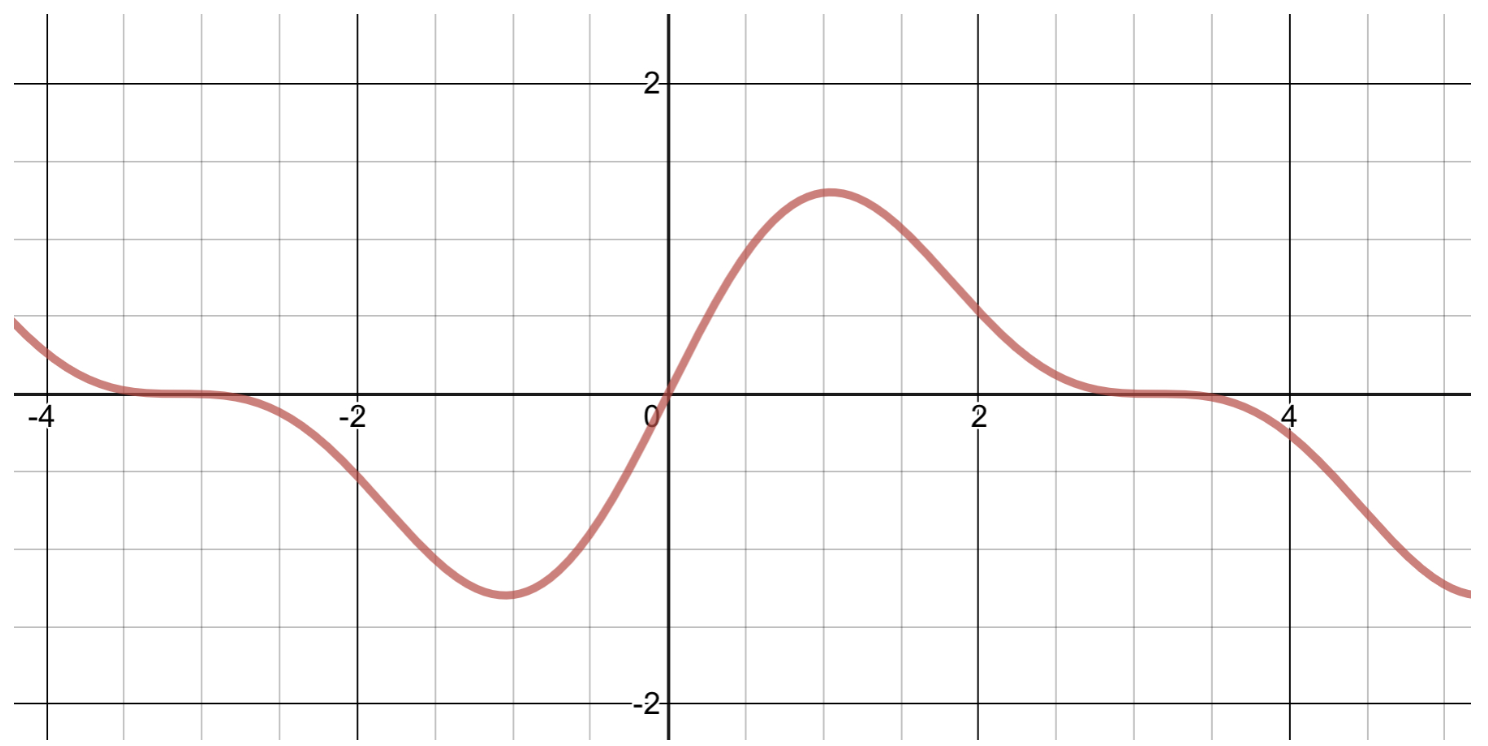
\includegraphics[scale=0.5]{D3graph1.png}
\vspace{.5in}
\item Calculate the indicated derivatives using derivative rules:\\


\begin{enumerate}
\item $\dfrac{d}{dx} \displaystyle{\frac{x^{-2}\sin(x)-\frac{1}{2}x^2}{\sin(x)\cos(x)}}=$

\end{enumerate}
\end{enumerate}
\end{document}
